\chapter{Data Acquision and Storage}\label{final}


\section{Data acquisition}
Data is acquired by accelerometer present in the smartphone. Data logging is triggered by the subject by pressing the start button and the smartphone is kept in the trouser’s pocket, in a fixed orientation. Such that the +Y axis, +Z axis and X axis of the smart phone points in top,forward,sideways direction respectively.\newline

Then the subject walks considerable distance with the phone kept in the pocket with each leg.
\section{Storage}

The data is saved in txt format, which can be easily read on the computer. Two options are provided for storing accelerometer data, either in internal storage or in the external storage.\newline

\begin{figure}
\center{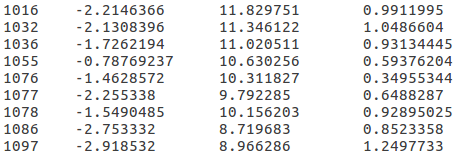
\includegraphics[width=100mm,scale=0.5]{pictures/recordedCrop.png}}
\caption{The first, second, third and  fourth columns of the data log files are time, X-axis, Y-axis and  Z-axis respectively.}
\end{figure}

Each time data is recorded the data log file is overwritten.
We use sensor delay fastest for logging data. All three axis reading are stored in the log file.\newline

The app can also be used for standalone data logger.\newline

Only Z-axis is used here for further analysis. In this orientation we could have used both Z and Y axis effectively, but using X-axis is avoided because the time series graph obtained doesn’t provide meaningful gait cycle feature template.\\

\begin{figure}
\center{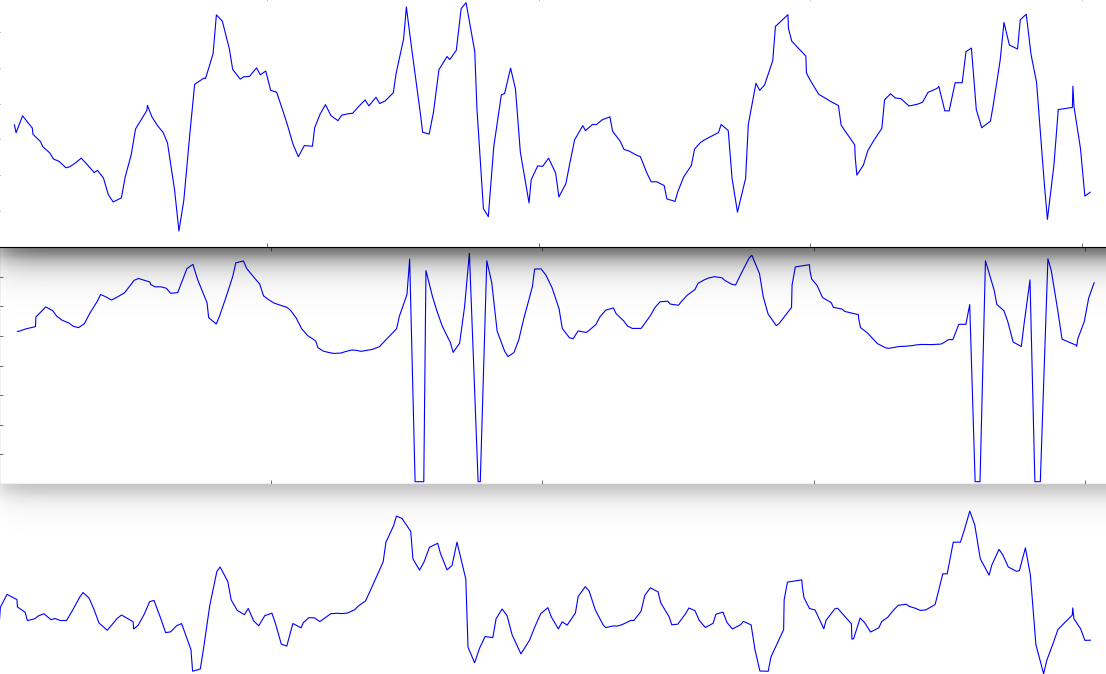
\includegraphics[scale=0.3]{pictures/XYZcrop.png}}\\[1.0cm]
\caption{Raw X, Y, Z axis readings, from top to bottom. }
\end{figure}

